% First draft: 1977_heilongjiang_preliminary_q11_fig1 (exact 120/45/15 triangle).
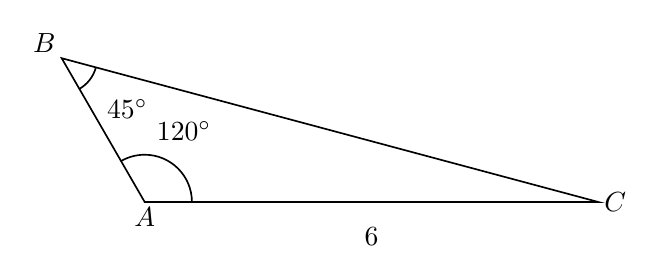
\begin{tikzpicture}[x=1cm,y=1cm,font=\normalsize,
 geometry edge/.style={solid,line width=.6pt},
 geometry mark/.style={solid,line width=.6pt},
 geometry label/.style={font=\normalsize,inner sep=2pt}]
\coordinate (A) at (0.0,0.0);
\coordinate (C) at (5.760000000000001,0.0);
\coordinate (B) at (-1.054153162899,1.825846837101);
\coordinate (L_120) at (0.5,0.9);
\coordinate (L_45) at (-0.22105899269420315,1.1867204995408431);
\coordinate (L_6) at (2.88,-0.25);
\draw[geometry edge] (A)--(B)--(C)--cycle;
\draw[geometry mark] (A) ++(0:6mm) arc[start angle=0,end angle=120,radius=6mm];
\draw[geometry mark] (B) ++(-60:4.5mm) arc[start angle=-60,end angle=-15,radius=4.5mm];
\node[geometry label,below] at (A) {$A$};
\node[geometry label,above left] at (B) {$B$};
\node[geometry label,right] at (C) {$C$};
\node[geometry label] at (L_120) {$120^\circ$};
\node[geometry label] at (L_45) {$45^\circ$};
\node[geometry label,below] at (L_6) {$6$};
\end{tikzpicture}
